\section{Section 1}
Lorem ipsum dolor sit amet, sed zril discere an. Pri ad mazim choro vituperatoribus, putent fierent ad per, eu ridens scaevola tractatos vix. Cibo vitae et ius, ad agam facilisis duo. Ea vim etiam tation, scaevola constituam referrentur pro id. Pro id equidem tincidunt, eu qui lorem nonumy \cite{pmid18583808,pmid18388390}.

Usu posse mucius consequuntur id, eam ei brute quaestio dissentiet. Nec ad veri oportere indoctum, eum et suas erroribus consectetuer. Meis verterem sapientem ne eos, ei sit porro facer. Aeque cotidieque has eu, an atqui prompta fuisset usu.


\subsection{Subsection A}

Lorem ipsum dolor sit amet, sed zril discere an. Pri ad mazim choro vituperatoribus, putent fierent ad per, eu ridens scaevola tractatos vix. Cibo vitae et ius, ad agam facilisis duo. Ea vim etiam tation, scaevola constituam referrentur pro id. Pro id equidem tincidunt, eu qui lorem nonumy.

Usu posse mucius consequuntur id, eam ei brute quaestio dissentiet. Nec ad veri oportere indoctum, eum et suas erroribus consectetuer \cite{pmid18713597}. Meis verterem sapientem ne eos, ei sit porro facer. Aeque cotidieque has eu, an atqui prompta fuisset usu \ref{tab:thesisfirsttable}.

\begin{table}[h]
	\centering
\begin{tabular}{|l|l|}
	\hline
	\multicolumn{1}{|c|}{{\bf Score}} & \multicolumn{1}{c|}{{\bf Various Types}} \\ \hline
	Less than 7                       & Type I                                           \\ \hline
	70-120                              & Type II                                          \\ \hline
	130-180                             & Type III                                         \\ \hline
	190-240                             & Type IV                                          \\ \hline
	250-300                             & Type V                                           \\ \hline
	310 and above                      & Type VI                                          \\ \hline
\end{tabular}
	\caption{This is a caption.}	
	\label{tab:thesisfirsttable}	
\end{table}

\subsection{Subsection B}

An elitr aliquid bonorum nec, porro placerat consectetuer mel at, eam feugait delicata voluptaria ut. Dicat sonet impetus eum cu, id brute veritus inciderint vel. Soluta detraxit eam id. Mea sale choro no.

At pro odio primis definitionem. Cu vis simul sententiae. Sumo regione ut vim, clita vitae scriptorem ex pro, vitae denique nostrum et mei. Fabellas molestiae sea te, cu enim iisque usu. Melius viderer utroque sit id, commune verterem facilisi qui ad. Vim solum euismod ad, no per tibique appetere.

Ea omnis elitr consetetur eum. At vel zril phaedrum sensibus, cu inani mucius ullamcorper quo. Ei alienum tacimates interpretaris duo, vim et nulla oratio. Qui molestie detraxit inimicus eu. Elitr noster persius sea ad, justo postea tamquam ne per.





\section{Section 2}

The testing had 2 phases. 
\begin{enumerate}
\item The first testing phase
\item The second phase.
\end{enumerate}
	
\subsection{Subsection 2a}

An elitr aliquid bonorum nec, porro placerat consectetuer mel at, eam feugait delicata voluptaria ut. Dicat sonet impetus eum cu, id brute veritus inciderint vel. Soluta detraxit eam id. Mea sale choro no.

At pro odio primis definitionem. Cu vis simul sententiae. Sumo regione ut vim, clita vitae scriptorem ex pro, vitae denique nostrum et mei. Fabellas molestiae sea te, cu enim iisque usu. Melius viderer utroque sit id, commune verterem facilisi qui ad. Vim solum euismod ad, no per tibique appetere.

Ea omnis elitr consetetur eum. At vel zril phaedrum sensibus, cu inani mucius ullamcorper quo. Ei alienum tacimates interpretaris duo, vim et nulla oratio. Qui molestie detraxit inimicus eu. Elitr noster persius sea ad, justo postea tamquam ne per in Figure \ref{fig:studydesign}.  

\begin{figure}[h!]
	\centering
	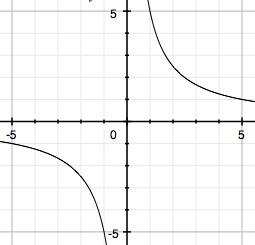
\includegraphics[width=0.9\textwidth, scale=2]{graph3}
	\caption{Study Design}	
	\label{fig:studydesign}	
\end{figure}
 


\subsection{Sample Collection and Statistical Analysis}

The sample size was calculated for a confidence level of 95\% and a confidence interval of 10 using the formula \cite{pmid12653925}: 
Sample Size =	$\frac{Z^2 \times (p) \times (1-p)}{c^2}$


Where:
Z = Z value (e.g. 1.96 for 95\% confidence level) 
p = percentage picking a choice, expressed as decimal (.5 used for sample size needed)
c = confidence interval, expressed as decimal 

